\documentclass[a4paper]{scrartcl}%{{{
\usepackage{float}
\usepackage{tikz}
\usetikzlibrary{arrows,automata}
\usepackage{pgf}
\usepackage[utf8]{inputenc} % this is needed for umlauts
\usepackage[ngerman]{babel} % this is needed for umlauts
\usepackage[T1]{fontenc}    % this is needed for correct output of umlauts in pd
\usepackage{amssymb}
\usepackage{amsmath}
\usepackage{mathabx}
\usepackage{mathrsfs}
\usepackage{dsfont}
\usepackage{wasysym}
\usepackage{graphicx}
\usepackage{fancyhdr}
\usepackage{lastpage}
\usepackage{imakeidx}
\setlength{\parskip}{\medskipamount}
\setlength{\parindent}{0pt}
\usepackage{enumitem}
\usepackage{hyperref}
\usepackage{verbatim}

%%%%%%%%%%%%%%%%%%%%%%%%
% Kopf- und Fusszeilen %
%%%%%%%%%%%%%%%%%%%%%%%%
\pagestyle{fancy}
\lhead{
        Maximilian Roth
}
\chead{Logik-Tutorat Lösungen Probeklausur\\}
\rhead{
    \begin{tabular}{rr}
        \today{} \\
        Seite \thepage{} von \pageref{LastPage}
    \end{tabular}
}
\lfoot{}
\cfoot{}
\rfoot{} 

%%%%%%%%%%%%%%%%%%%%%%%%
% Anfang des Dokuments %
%%%%%%%%%%%%%%%%%%%%%%%%%
\begin{document}
\section*{Disclaimer}
\label{sec:disclaimer}
Auch in diesem Dokument können sich Fehler befinden!\\
Sie sind nicht die Musterlösung der Aufgaben, sondern selbst erstellte Lösungen.\\

Als generelle Lektüre kann ich nur das Skript von Markus Junker aus dem WS 17/18 empfehlen:\\
\url{http://home.mathematik.uni-freiburg.de/junker/skripte/InfoLogik.pdf}\\
Hier ist vieles sehr genau und verständlich erklärt.
%}}}

\section*{}%
\label{sec:aufgabe_6}

    \begin{figure}[H]
        \centering
        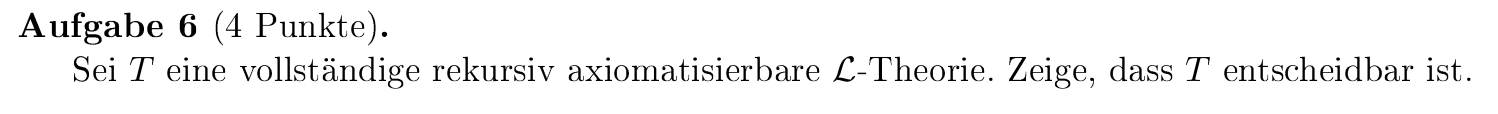
\includegraphics[scale=0.3]{./A-6.png}
        \label{fig:./A-6}
    \end{figure}

    \underline{ZZ:} Sei T vollständig und rekursiv axiomatisierbar.\\
    Zeige, dass T entscheidbar.\\

    Damit T entscheidbar ist muss $\{\lceil \varphi \rceil | T \vdash \varphi \}$ rekursiv sein (Def. 3.30).\\
    Dafür wiederum müssen die folgenden Mengen rekursiv \underline{aufzählbar} sein.\\
    \begin{itemize}
        \item $\{\lceil \varphi \rceil | T \vdash \varphi \}$ rekursiv aufzählbar\\
            Folgt aus Lemma 3.32 (\ref{fig:./L-3-32}), da T rek. axiomatisierbar\\
        \item $\mathds{N} \backslash \{\lceil \varphi \rceil | T \vdash \varphi \}$\\
            $= \mathds{N} \backslash \{\lceil \varphi \rceil | \varphi \text{ Aussage}\} \cup \{\lceil \varphi \rceil | T \vdash \neg \varphi\}$ (T vollständig)\\
            \\Wir zeigen, dass jeder Teil rekursiv aufzählbar ist:\\
            \begin{itemize}
                \item $ \mathds{N} \backslash \{\lceil \varphi \rceil | \varphi \text{ Aussage}\}$ ist rekursiv aufzählbar,\\
                    da letzteres nach Lemma 3.28 (\ref{fig:./L-3-28}) primitiv \underline{rekursiv} ist und damit auch das komplement rekursiv aufzählbar ist.\\
                \item $\{\lceil \varphi \rceil | T \vdash \neg \varphi\}$\\
                    $= \{\lceil \varphi \rceil | \varphi \text{ Aussage}\} \cap \{n \in \mathds{N} | f(n) \in \{\lceil \varphi \rceil | T \vdash \varphi\}\}$\\
                    Wobei $f: \mathds{N} \rightarrow \mathds{N}, \text{ rekursiv mit } f(\lceil \varphi \rceil) = \lceil \neg \varphi \rceil$\\
                    Die Aussagen, deren Negat in T wahr ist.\\
                    \\Wir wissen bereits, dass $\{\lceil \varphi \rceil | \varphi \text{ Aussage}\}$ rekursiv aufzählbar ist, fehlt also nur noch:\\
                    \\$M = \{n \in \mathds{N} | f(n) \in \{\lceil \varphi \rceil | T \vdash \varphi\}\}$\\
                    \\Nach Lemma 3.22 (\ref{fig:./L-3-22}) müssen wir nur eine Fkt. $x: \mathds{N} \rightarrow \mathds{N}$ finden,\\
                    so dass gilt Im(x) = M, damit M rekursiv aufzählbar ist.\\
                    \\Da $\{\lceil \varphi \rceil | T \vdash \varphi\}$ rekursiv \underline{aufzählbar} ist folgt:\\
                    $\overset{Lemma 3.22 (\ref{fig:./L-3-22})}{\Rightarrow} \exists \text{rekursive Fkt. } g: \mathds{N} \rightarrow \mathds{N}:
                    Im(g) = \{\lceil \varphi \rceil | T \vdash \varphi\}$\\
                    \\Sei nun h rekursiv wie folgt:\\
                    $h: \mathds{N}^2 \rightarrow \mathds{N},\\
                    h(n,m) = \begin{cases}
                        n, &\text{ falls }f(n) = g(m)\\
                        \psi, &\text{ sonst}\\
                    \end{cases}$\\
                    Wobei $\psi$ fest und $\psi \in \{n \in \mathds{N} | f(n) \in \{\lceil \varphi \rceil | T \vdash \varphi\}\}$\\
                    \\$Im(h) = M = \{n \in \mathds{N} | f(n) \in \{\lceil \varphi \rceil | T \vdash \varphi\}\}$, da:\\
                    \begin{itemize}
                        \item $\psi \in M$\\
                        \item n nur im Bild ist, wenn $\neg f(n) \in Img(g) = \{\lceil \varphi \rceil | T \vdash \varphi\}$ und damit
                    $n \in M = \{n \in \mathds{N} | f(n) \in \{\lceil \varphi \rceil | T \vdash \varphi\}\}$.\\
                    \end{itemize}
                    Allerdings muss für die Fkt. $x$ gelten, dass $x: \mathds{N} \rightarrow \mathds{N}$, aber $h: \mathds{N}^2 \rightarrow \mathds{N}$\\
                    D.h. wir brauchen noch eine rekursiv aufzählbare bijektive Fkt. $i: \mathds{N} \rightarrow \mathds{N}^2$\\
                    \\Dann ist $x = h \circ i: \mathds{N} \rightarrow \mathds{N}$ rekursiv aufzählbar und\\
                    $Im(h \circ i) = \{n \in \mathds{N} | f(n) \in \{\lceil \varphi \rceil | T \vdash \varphi\}\}$\\
                    \\$\Rightarrow$ M ist rekursiv aufzählbar\\
            \end{itemize}
            Jeder Teil ist rekursiv aufzählbar $\Rightarrow$ $\mathds{N} \backslash \{\lceil \varphi \rceil | T \vdash \varphi \}$ ist rekursiv aufzählbar.\\
    \end{itemize}
    $\Rightarrow$ $\{\lceil \varphi \rceil | T \vdash \varphi \}$ ist rekursiv.\\
    \\$\Rightarrow$ T ist entscheidbar.\

    

    \begin{figure}[H]
        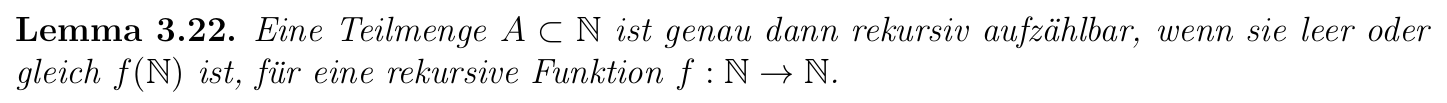
\includegraphics[scale=0.3]{./L-3-22.png}
        \caption{Lemma 3.22}
        \label{fig:./L-3-22}
    \end{figure}
    \begin{figure}[H]
        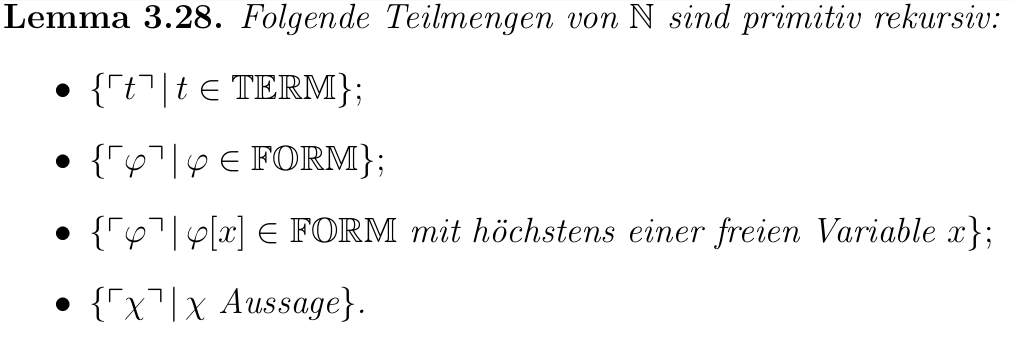
\includegraphics[scale=0.3]{./L-3-28.png}
        \caption{Lemma 3.28}
        \label{fig:./L-3-28}
    \end{figure}
    \begin{figure}[H]
        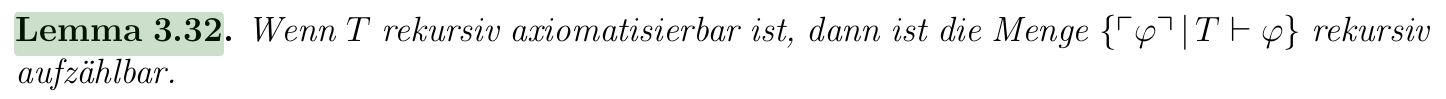
\includegraphics[scale=0.3]{./L-3-32.png}
        \caption{Lemma 3.32}
        \label{fig:./L-3-32}
    \end{figure}
    
    
    



\end{document}
